\documentclass[titlepage]{tfg-ucm}
\usepackage[english,spanish,es-tabla]{babel}
\usepackage[utf8]{inputenc}
\usepackage{lipsum}
\usepackage{geometry} %% Remove showframe in your document
\usepackage{biblatex}
\usepackage{import}
\usepackage{minted}
\usepackage{xargs}
\usepackage{tabularx}
\usepackage{hyperref}
\usepackage{subcaption}
% \usepackage[spanish,colorinlistoftodos,prependcaption,textsize=footnotesize]{todonotes}
\usepackage{enumitem}
\usepackage{wrapfig}
\usepackage{subcaption}
\usepackage{csquotes}

\title{Implementación de una red en chip en un procesador RISC-V}
\author{David Davó Laviña}
\englishTitle{NoC implementation of a RISC-V processor}
\director{Óscar Garnica Alcázar}
\codirector{Juan Lanchares Dávila}
\cursoAcademico{2021-2022}
\facultad{Facultad de Informática}
\departamento{Departamento de Arquitectura de Computadores y Automática}
\universidad{Universidad Complutense de Madrid}
\asignatura{Trabajo de Fin de Grado del Grado en Ingeniería Informática}
\universityLogo{./images/logos/EscudoUCMTransparenteBig.png}
\date{\today}

\DeclareBibliographyCategory{cited}
\AtEveryCitekey{\addtocategory{cited}{\thefield{entrykey}}}

%% HYPHENATION EXCEPTIONS (tell LaTeX how to)
% \uchyph=0 % Don't hyphenate acronyms (creates a lot of overfulls)

% https://tex.stackexchange.com/questions/65355/flushbottom-vs-raggedbottom
% This eliminated the undeful thing
\raggedbottom

% Fixes the problem when having repeated chapter numbers
% From https://tex.stackexchange.com/questions/146254/how-to-repeat-chapter-numbers
% We have to use \chaptertype{E} inside the otherlanguage environment so when we use \chapter
% the href will be created as E# instead of just # (already used by the spanish version).
\newcommand{\chaptype}{}
\newcommand{\chaptertype}[1]{\renewcommand{\chaptype}{#1}}
\renewcommand{\theHchapter}{\chaptype\arabic{chapter}}

\addbibresource{bibliografia.bib}

%% TODO & ANNOTATION COMMANDS
% We use newcommandx to be able to pass xkeyvals to the todo command
\newcommandx{\tdinquiry}[2][1=]{\todo[linecolor=ProcessBlue,backgroundcolor=ProcessBlue!25,bordercolor=ProcessBlue,#1]{#2}}
\newcommandx{\tdcorrect}[2][1=]{\todo[linecolor=Red,backgroundcolor=Red!25,bordercolor=Red,#1]{#2}}
%% --------------------------

%% FROM RISC-V ISA MANUAL
\newcommand{\instbit}[1]{\mbox{\scriptsize #1}}
\newcommand{\instbitrange}[2]{~\instbit{#1} \hfill \instbit{#2}~}
%% ---------------------

\begin{document}

% Como estas páginas no cuentan, usamos números Romanos en lugar de Arábigos
\frontmatter
\makecover

% \makefirstpage
% \import{chapters}{autorizacion}

\import{chapters}{agradecimientos}

\import{chapters}{resumen}
\import{chapters}{abstract}

\setcounter{tocdepth}{1}
\tableofcontents

% \cleardoublepage
% {
%     \let\cleardoublepage\relax
    \listoffigures
    A menos que se especifique lo contrario, las figuras de este documento son de autoría propia y siguen la licencia de este documento.
    \listoftables
% }

\mainmatter
\part{Introducción}
\import{chapters/introduccion}{motivaciones}
\import{chapters/introduccion}{objetivos}

\part{Estado del arte}
\import{chapters/estado_del_arte}{risc-v}
\import{chapters/estado_del_arte}{noc}

\part{Diseño e implementación}
% \section{Elección del núcleo RISC-V}
\label{sec:desCore}

Para seleccionar el núcleo (\textit{core}) a modificar, se ha explorado la lista de \textit{cores} de RISC-V Exchange \cite{RiscVExchangeCores}. El objetivo principal ha sido buscar un proyecto en el que fuese sencillo embeber una NoC como prueba de concepto, sin importar mucho las características técnicas del procesador, su potencia o sus resultados en \textit{benchmarks}. Por lo tanto, hemos priorizado que su lenguaje de programación fuese conocido, tuviese licencias abiertas, y una amplia documentación y herramientas de desarrollo.

Se ha filtrado la selección buscando Cores escritos en lenguajes conocidos (VHDL o SystemVerilog) y con licencia libre reconocida por OSI (Apache, BSD, GPL o MIT) \cite{OSILicenses}. Finalmente, la selección se redujo a los siguientes núcleos:

\begin{description}
    \item[SweRV Core EH1] [RV32IMCZ]: Es superescalar con 2 vías de lanzamiento (dual issue) y segmentación en 9 fases. Ha sido fabricado en tecnología de 28nm, pero cuenta con optimizaciones para FPGA. Creado por Western Digital. Tiene 4 unidades aritmético-lógicas (ALU), 2 \textit{early} y 2 \textit{late}, cada una conectada a una de las vías del ILP \cite{RepoSwervEH1}.
    \item[SweRV Core EH2] [RV32IMACZ]: Basado en el EH1, se le añade multithreading para 2 hilos, y por lo tanto también se le agregan instrucciones atómicas \cite{RepoSwervEH2}.
    \item [SweRV Core EL2] [RV32IMC]: Es un núcleo mucho más sencillo que el EH1 creado para reemplazar a las máquinas de estados y otras funciones lógicas implementadas en Sistema en Chip (haciendo que puedan ser actualizadas). La segmentación es en solo 4 etapas y es escalar \cite{RepoSwervEL2}.
    \item [biRISC-V] [RV32IMZicsr]: Superescalar con dual issue y segmentación en 6-7 etapas, tiene un divisor hardware, 1 unidad de load-store y 2 ALUs. Implementa también instrucciones privilegiadas, por lo que puede ejecutar sistemas operativos de propósito general \cite{RepoBiRISCV}.
    \item [PicoRV32] [RV32IMC]: Es un pequeño procesador de menos de 2000 LUTs, por lo que caben múltiples en una FPGA. % Una idea alternativa hubiese sido crear una interfaz de red para este procesador, y conectar varios de ellos en una FPGA formando un SoC manycore \cite{PicoRV32gh}.
\end{description}

Algunos otros núcleos y herramientas que se consideraron y fueron descartados en fases tempranas (principalmente por el lenguaje de programación o su complejidad) fueron los siguientes:

\begin{description}
    \item [WARP-V] Está escrito en TL-Verilog y es un generador de cores con muchas opciones de configuración. Parte de este trabajo podría haber sido añadir al WARP-V la opción de usar una NoC, al igual que existen opciones para añadir o quitar etapas del pipeline.
    \item [Rocket Chip] Más que un procesador, se trata de un generador escrito en \textbf{Chisel}, lenguaje libre de definición de hardware basado en Scala que emite código sintetizable en Verilog. Ha sido diseñado por el departamento de D. Patterson, A. Waterman y K. Asanović, creadores del RISC-V. \cite{AsanovicRocketChip}.
    \item [BOOM] [RV64GC] \textit{Berkeley Out-of-Order Machine}. Está creado por el mismo departamento que Rocket y con herramientas muy similares. Su característica principal es su alto grado de paralelismo a nivel de instrucción. Sin embargo, su estructura es mucho más compleja y, por lo tanto, difícil de modificar \cite{Celio:EECS-2015-167}.
\end{description}

La principal ventaja de Rocket y BOOM es que, debido a su longevidad y soporte a lo largo del tiempo, cuentan con amplia documentación, literatura, herramientas, y han sido implementados tanto en FPGA como en ASICs, por lo que aunque no han sido usados directamente en este proyecto, sí que se ha consultado en ocasiones literatura relacionada con estos procesadores.

\begin{figure}[h]
    \centering
    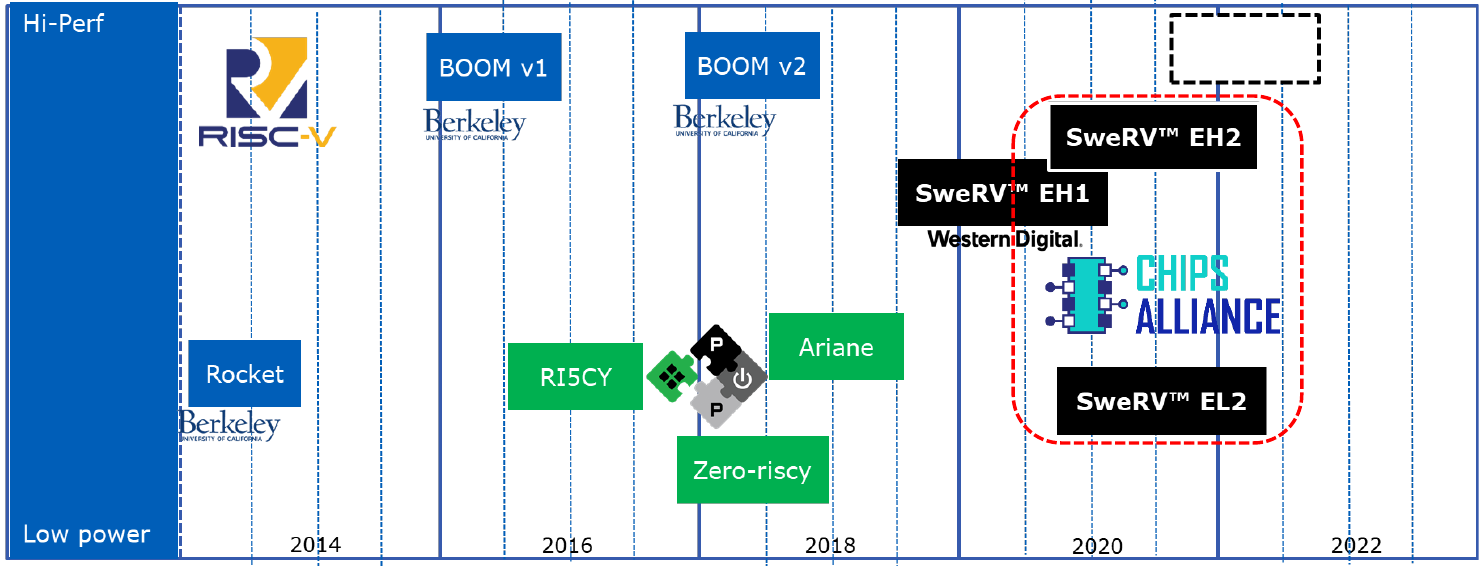
\includegraphics[width=\linewidth]{images/external/roadmap_compare.png}
    \caption[Comparativa de la potencia de varios Cores RISC-V de código abierto]{Comparativa de la potencia de varios Cores RISC-V de código abierto. Resaltado en rojo los procesadores de la familia SweRV. Extraído de \citetitle{SweRVRoadmap}~\cite{SweRVRoadmap}.}
    \label{fig:swerv_comparative}
\end{figure}

Finalmente, se eligió la familia SweRV debido a la familiaridad con el proyecto (se usa este procesador en la actividad formativa ``Implementación ASIC de 28nm del procesador RISC V"). En la figura \ref{fig:swerv_comparative} se muestra una comparativa de dichos procesadores con otros cores de código abierto. Dentro de los procesadores de esta familia, se decidió modificar el EL2 por su sencillez y los pocos recursos humanos de los que se dispone en este proyecto. No obstante, tratándose de una prueba de concepto, siempre es posible en el futuro aplicar las técnicas aprendidas a otros productos más complejos, con mejoras y optimizaciones.

\import{chapters/diseño}{tecnologias_metodologias}
\import{chapters/diseño}{rtl}
\import{chapters/diseño}{problemas}

\part{Conclusiones y resultados}
\import{chapters/conclusiones}{noc}
\import{chapters/conclusiones}{swerv}
\import{chapters/conclusiones}{trabajo_futuro}
\import{chapters/conclusiones}{conclusiones}

% \todo[disable]{Eliminar la lista de TODOs}
% \listoftodos

\nocite{Kamali2015TowardsArchitectures}
\nocite{DeMicheli2006NetworksTools}
\nocite{Jantsch2003NetworksChip}
\nocite{Asanovic2014InstructionRISC-V}
\nocite{Chen2016RISC-VGeneology}
\printbibliography

% \nocite{*}
% \printbibliography[notcategory=cited]

% \part{Anexos}

\end{document}
